% \documentclass{standalone}
% \usepackage{tikz}
% \begin{document}
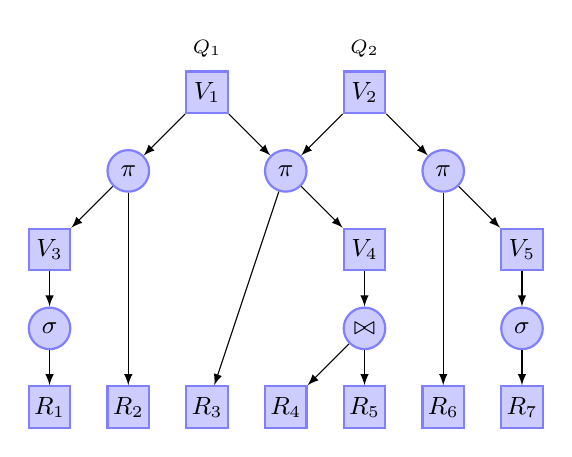
\begin{tikzpicture}[
every node/.style  = {fill=blue!20,draw=blue!50,thick,
	minimum size=1.5em,inner sep=0pt,font=\small},
circle_node/.style={circle},
rec_node/.style={rectangle},
edge from parent/.style={->,draw},
every label/.append style={font=\scriptsize},
>=latex]
  
    \node[rec_node] (r1) at (0, 0) {$R_1$};
    \node[rec_node] (r2) at (1, 0)  {$R_2$};
    \node[rec_node] (r3) at (2, 0) {$R_3$};
	\node[rec_node] (r4) at (3, 0) {$R_4$};
	\node[rec_node] (r5) at (4, 0) {$R_5$};
	\node[rec_node] (r6) at (5, 0) {$R_6$};
	\node[rec_node] (r7) at (6, 0) {$R_7$};
	
	\node[circle_node] (op1) at (0, 1) {$\sigma$};
	\node[circle_node] (op2) at (4, 1) {$\bowtie$};
	\node[circle_node] (op3) at (6, 1) {$\sigma$};
	
	\node[rec_node] (v3) at (0, 2) {$V_3$};
	\node[rec_node] (v4) at (4, 2) {$V_4$};
	\node[rec_node] (v5) at (6, 2) {$V_5$};
	
	\node[circle_node] (op4) at (1, 3) {$\pi$};
	\node[circle_node] (op5) at (3, 3) {$\pi$};
	\node[circle_node] (op6) at (5, 3) {$\pi$};
	
	\node[rec_node,label={\scriptsize $Q_1$}] (v1) at (2, 4) {$V_1$};
	\node[rec_node,label={\scriptsize $Q_2$}] (v2) at (4, 4) {$V_2$};


    \draw[->] (v1) -- (op4);
	\draw[->] (v1) -- (op5);
	\draw[->] (v2) -- (op5);
	\draw[->] (v2) -- (op6);
	
	\draw[->] (op4) -- (v3);
	\draw[->] (op4) -- (r2);
	\draw[->] (op5) -- (v4);
	\draw[->] (op5) -- (r3);
	\draw[->] (op6) -- (v5);
	\draw[->] (op6) -- (r6);
	
	\draw[->] (v3) -- (op1);
	\draw[->] (v4) -- (op2);
	\draw[->] (v5) -- (op3);
	
	\draw[->] (op1) -- (r1);
	\draw[->] (op2) -- (r4);
	\draw[->] (op2) -- (r5);
	\draw[->] (op3) -- (r7);
	
\end{tikzpicture}
%\end{document}
